% \section{Related Work}

% \subsection{Medical Segmentation and Lightweight U-Shaped Networks}

% U-Net~\cite{ronneberger2015unet} and its encoder--decoder variants remain a primary template for medical image segmentation because skip connections combine deep semantic features with spatially precise reconstruction. Task-specific methods strengthen this template through mechanisms such as reverse attention in PraNet~\cite{fan2020pranet} and uncertainty-aware context attention in UACANet~\cite{kim2021uacanet}. TransUNet~\cite{chen2021transunet} instead introduces a Transformer encoder to enlarge the receptive field through global self-attention. These approaches establish the value of contextual reasoning, but their attention modules or pretrained encoders can be costly when the deployment budget is limited.
% Lightweight U-shaped networks reduce this cost through compact channel schedules and efficient local operators. UNeXt~\cite{valanarasu2022unext} combines convolution with shifted MLP blocks, CMUNeXt~\cite{tang2024cmunext} uses large kernels and skip fusion, EGE-UNet~\cite{ruan2023egeunet} develops group-enhanced attention, and EMCAD~\cite{rahman2024emcad} employs efficient multi-scale convolutional decoding. MK-UNet~\cite{rahman2025mkunet} further uses parallel multi-kernel depth-wise convolutions, channel shuffle, and lightweight decoder attention to capture multi-scale boundary evidence.

% \subsection{Visual State-Space Models}

% State-space models offer an efficient alternative to self-attention for long-range dependency modeling. Mamba~\cite{gu2023mamba} uses input-dependent state transitions with linear sequence complexity, while VMamba~\cite{liu2024vmamba} extends selective scanning to visual feature maps through multiple two-dimensional traversal directions. VM-UNet~\cite{ruan2024vmunet} incorporates visual state-space blocks into a U-shaped segmentation architecture. For lightweight medical segmentation, UltraLight VM-UNet~\cite{wu2024ultralight} further reduces Vision Mamba cost by partitioning deep features into parallel channel groups and processing them with parallel Vision Mamba branches.
% In grouped multi-directional scans, direction--group branches are typically processed independently and merged only after selective scanning. This design can limit information exchange across traversal directions and channel subspaces before fusion.

% \subsection{Foundation-Model Distillation for Lightweight Segmentation}

% Strong Transformer encoders and vision foundation models provide rich semantic representations for medical image segmentation. Swin Transformer~\cite{liu2021swin} and its medical segmentation variant Swin-Unet~\cite{cao2022swinunet} model hierarchical visual features, while DINOv3~\cite{simeoni2025dinov3} provides dense features through large-scale self-supervised pretraining. However, directly deploying such large encoders conflicts with the parameter, memory, and latency budgets of lightweight systems.

% Feature-level distillation offers a practical alternative: a frozen teacher provides dense supervision only during training, allowing a compact student to inherit semantic context without the teacher's deployment cost~\cite{hinton2015distilling}. Most distillation settings use a fixed distillation coefficient. However, a fixed coefficient cannot adapt to the dynamic state of optimization: as training progresses, the gradient contribution of the teacher-supervised deep student feature to the overall network can change, so the same coefficient may yield insufficient teacher supervision or impose an overly strong constraint on the primary task objective.
% To address this dynamic balancing problem, RT-DETRv4~\cite{liao2025rtdetrv4} proposes a gradient-aware distillation strategy for real-time detection. In its reported configuration, a frozen DINOv3-ViT-B teacher supervises deep detector features through a Deep Semantic Injector. Its Gradient-guided Adaptive Modulation adjusts the semantic-transfer strength using gradient norm ratios, enabling teacher supervision to remain coordinated with the detection objective as the optimization state evolves.





% \section{Related Work}

% \subsection{Medical Segmentation and Lightweight U-Shaped Networks}

% Medical image segmentation has been widely studied due to its importance in computer-aided diagnosis and clinical decision support. U-Net~\cite{ronneberger2015unet} established a simple yet effective encoder--decoder framework with skip connections, enabling the decoder to recover spatial details from high-resolution encoder features. Based on this paradigm, many methods have been proposed to improve medical segmentation by enhancing contextual aggregation, attention modeling, boundary refinement, and multi-scale feature fusion. For example, PraNet~\cite{fan2020pranet} introduces parallel partial decoding and reverse attention for polyp segmentation, while UACANet~\cite{kim2021uacanet} incorporates uncertainty-aware context attention to refine ambiguous regions. Transformer-based methods, such as TransUNet~\cite{chen2021transunet}, further introduce global self-attention to improve long-range feature interaction.

% Although these methods improve segmentation accuracy, their computational cost can limit practical deployment, especially in point-of-care or resource-constrained scenarios. This has motivated the development of lightweight U-shaped segmentation networks. UNeXt~\cite{valanarasu2022unext} combines convolutional stages with efficient tokenized MLP blocks. CMUNeXt~\cite{tang2024cmunext} explores large-kernel convolution and compact multi-scale feature extraction. EGE-UNet~\cite{ruan2023egeunet} and EMCAD~\cite{rahman2024emcad} further improve efficiency through lightweight decoding and attention mechanisms. More recently, MK-UNet~\cite{rahman2025mkunet} employs multi-kernel depth-wise convolution, channel shuffle, and lightweight decoder attention to capture multi-scale boundary evidence with low computational overhead. These designs are effective for local detail preservation, but lightweight CNN-dominated architectures still rely mainly on local operators and may lack explicit long-range contextual modeling. This motivates the integration of efficient global modeling mechanisms into compact U-shaped networks.

% \subsection{Visual State-Space Models}

% State-space models have recently attracted increasing attention as an efficient alternative to attention-based global modeling. Mamba~\cite{gu2023mamba} introduces an input-dependent selective state-space mechanism for sequence modeling with linear complexity. VMamba~\cite{liu2024vmamba} extends this idea to visual recognition by applying selective scanning to two-dimensional feature maps, enabling efficient long-range dependency modeling without the quadratic complexity of self-attention. In medical image segmentation, VM-UNet~\cite{ruan2024vmunet} incorporates visual state-space blocks into a U-shaped architecture, showing the potential of Mamba-like models for dense prediction tasks.

% Despite their efficiency, directly applying Vision Mamba blocks to segmentation networks can still introduce non-negligible computational cost, especially when high-dimensional features are processed. To address this issue, UltraLight VM-UNet~\cite{wu2024ultralight} partitions deep features into multiple channel groups and processes them with parallel Vision Mamba branches, reducing the cost of global modeling. However, most grouped scanning designs treat scan directions and channel groups as independent branches before fusion. Although this strategy reduces computation, it does not explicitly model the structural relationship between traversal directions and channel subspaces. As a result, complementary directional cues and group-wise semantic responses cannot be exchanged before multi-directional aggregation. Different from existing grouped selective scanning methods, our work introduces graph-based direction--group interaction inside the selective-scan block to alleviate this representation-isolation issue.

% \subsection{Foundation-Model Supervision for Compact Models}

% Large-scale foundation models have demonstrated strong representation ability across a wide range of visual tasks. In particular, DINOv3~\cite{simeoni2025dinov3} provides powerful semantic features learned from large-scale self-supervised pretraining. However, directly deploying such large pretrained models is often impractical for lightweight medical image segmentation because of their high computational and memory requirements. A more practical strategy is to use foundation models only during training, transferring their semantic knowledge to a compact student network while keeping the deployed model lightweight.

% Knowledge distillation provides a common framework for transferring information from a strong teacher model to a smaller student model. In dense prediction tasks, feature-level distillation is especially useful because it can provide spatially structured semantic supervision. Recent real-time detection work, such as RT-DETRv4~\cite{liao2025rtdetrv4}, shows that frozen DINOv3 features can serve as effective semantic supervision, and that the transfer strength can be adjusted according to gradient statistics. Different from detection-oriented designs, we adapt this training-time foundation-model supervision strategy to lightweight medical image segmentation. Specifically, the frozen DINOv3 teacher is aligned with a deep decoder representation of the student, and Gradient-Adaptive Distillation is used to regulate the semantic transfer strength during optimization. Since the teacher and projection head are discarded during inference, this supervision strategy enhances the compact student without increasing deployment cost.



\section{Related Work}

\subsection{Medical Segmentation and Lightweight U-Shaped Networks}

U-Net~\cite{ronneberger2015unet} and its encoder--decoder variants remain a primary template for medical image segmentation because skip connections combine deep semantic features with spatially precise reconstruction. Task-specific methods strengthen this template through mechanisms such as reverse attention in PraNet~\cite{fan2020pranet} and uncertainty-aware context attention in UACANet~\cite{kim2021uacanet}. TransUNet~\cite{chen2021transunet} instead introduces a Transformer encoder to enlarge the receptive field through global self-attention. These approaches establish the value of contextual reasoning, but their attention modules or pretrained encoders can be costly when the deployment budget is limited.

Lightweight U-shaped networks reduce this cost through compact channel schedules and efficient local operators. UNeXt~\cite{valanarasu2022unext} combines convolution with shifted MLP blocks, CMUNeXt~\cite{tang2024cmunext} uses large kernels and skip fusion, EGE-UNet~\cite{ruan2023egeunet} develops group-enhanced attention, and EMCAD~\cite{rahman2024emcad} employs efficient multi-scale convolutional decoding. MK-UNet~\cite{rahman2025mkunet} further uses parallel multi-kernel depth-wise convolutions, channel shuffle, and lightweight decoder attention to capture multi-scale boundary evidence. These lightweight CNN-based designs are effective for preserving local details, but they still mainly rely on local operators and may lack explicit long-range contextual modeling.

\subsection{Visual State-Space Models}

State-space models offer an efficient alternative to self-attention for long-range dependency modeling. Mamba~\cite{gu2023mamba} uses input-dependent state transitions with linear sequence complexity, while VMamba~\cite{liu2024vmamba} extends selective scanning to visual feature maps through multiple two-dimensional traversal directions. VM-UNet~\cite{ruan2024vmunet} incorporates visual state-space blocks into a U-shaped segmentation architecture. For lightweight medical segmentation, UltraLight VM-UNet~\cite{wu2024ultralight} further reduces Vision Mamba cost by partitioning deep features into parallel channel groups and processing them with parallel Vision Mamba branches.

In grouped multi-directional scans, direction--group branches are typically processed independently and merged only after selective scanning. Although this design reduces computation, it does not explicitly model the structural relationship between traversal directions and channel subspaces. This can limit the exchange of complementary directional cues and group-wise semantic responses before fusion.

\subsection{Foundation-Model Distillation for Lightweight Segmentation}

Strong Transformer encoders and vision foundation models provide rich semantic representations for medical image segmentation. Swin Transformer~\cite{liu2021swin} and its medical segmentation variant Swin-Unet~\cite{cao2022swinunet} model hierarchical visual features, while DINOv3~\cite{simeoni2025dinov3} provides dense features through large-scale self-supervised pretraining. However, directly deploying such large encoders conflicts with the parameter, memory, and latency budgets of lightweight systems.

Feature-level distillation offers a practical alternative: a frozen teacher provides dense supervision only during training, allowing a compact student to inherit semantic context without the teacher's deployment cost~\cite{hinton2015distilling}. Most distillation settings use a fixed distillation coefficient. However, a fixed coefficient cannot adapt to the dynamic state of optimization: as training progresses, the gradient contribution of the teacher-supervised deep student feature to the overall network can change, so the same coefficient may yield insufficient teacher supervision or impose an overly strong constraint on the primary task objective.

To address this dynamic balancing problem, RT-DETRv4~\cite{liao2025rtdetrv4} proposes a gradient-aware distillation strategy for real-time detection. In its reported configuration, a frozen DINOv3-ViT-B teacher supervises deep detector features through a Deep Semantic Injector, and Gradient-guided Adaptive Modulation adjusts the semantic-transfer strength using gradient norm ratios. Inspired by this strategy, our work adapts DINOv3-based gradient-adaptive distillation to lightweight medical image segmentation, where teacher features are aligned with a deep decoder representation and discarded during inference.






\begin{figure*}[t]
    \centering
    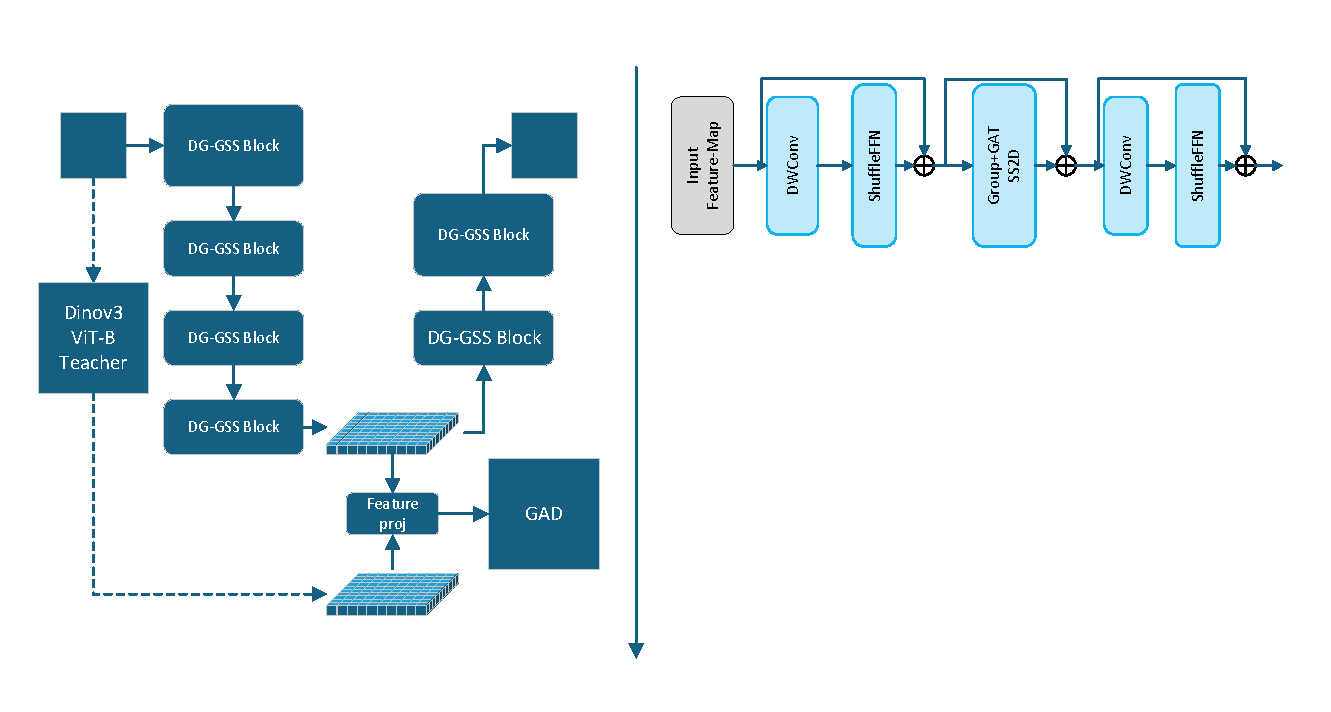
\includegraphics[width=\textwidth]{all-network.pdf}
    \caption{Overall architecture of GAD-MambaUNet. High-resolution stages retain multi-kernel local modeling, whereas deep stages use grouped state-space blocks with DG-GSS. During training, a frozen DINOv3 teacher supervises the first decoder block and GAD regulates the distillation coefficient according to its gradient share. The teacher and projection head are removed at inference.}
    \label{fig:overall-network}
\end{figure*}